\section{Introduction} \label{introduction}
\begin{figure}[tb]
  \centering
  \begin{subfigure}{0.6\linewidth}
  \begin{subfigure}{1\linewidth}
    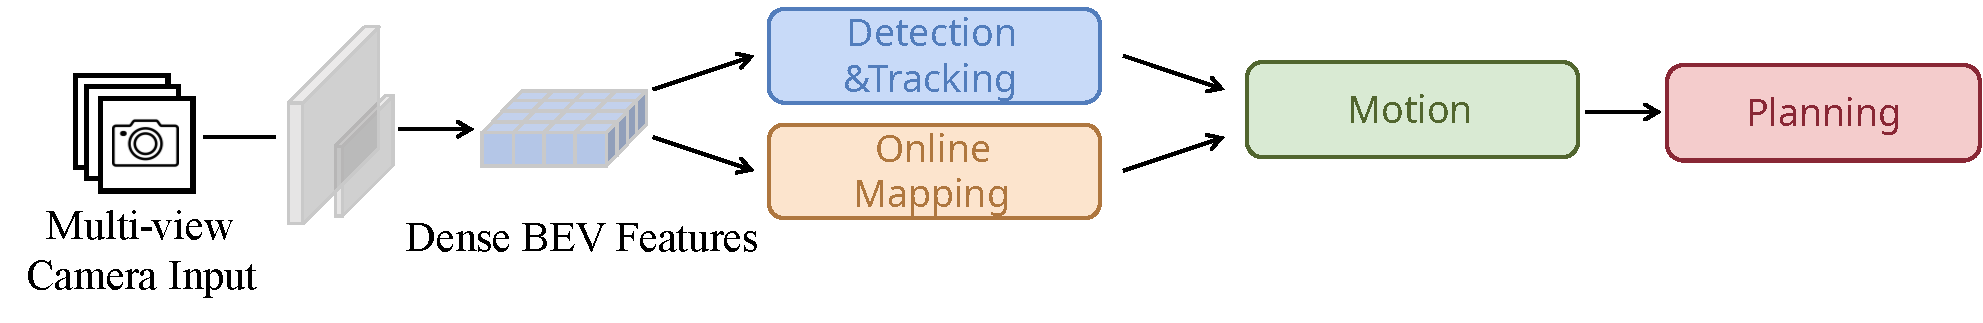
\includegraphics[width=1\linewidth]{Figures/pipeline_bev.pdf}
    \caption{BEV-Centric paradigm.}
    \label{fig:pipeline_bev}
  \end{subfigure}
  \hfill
  \\
  \begin{subfigure}{1\linewidth}
    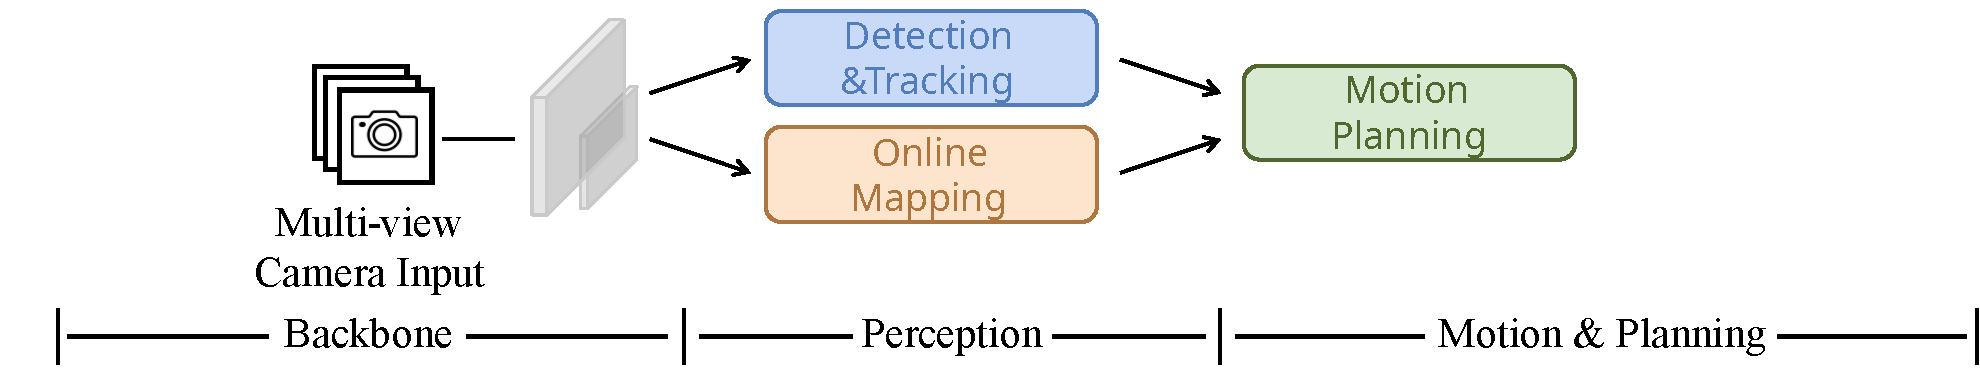
\includegraphics[width=1\linewidth]{Figures/pipeline_sparse.pdf}
    \caption{Sparse-Centric paradigm.}
    \label{fig:pipeline_sparse}
  \end{subfigure}
  \label{fig:short}
  \\
  \hfill
  \end{subfigure}
  \hspace{2pt}
  \begin{subfigure}{0.38\linewidth}
  \centering
    \begin{subfigure}{1\linewidth}
    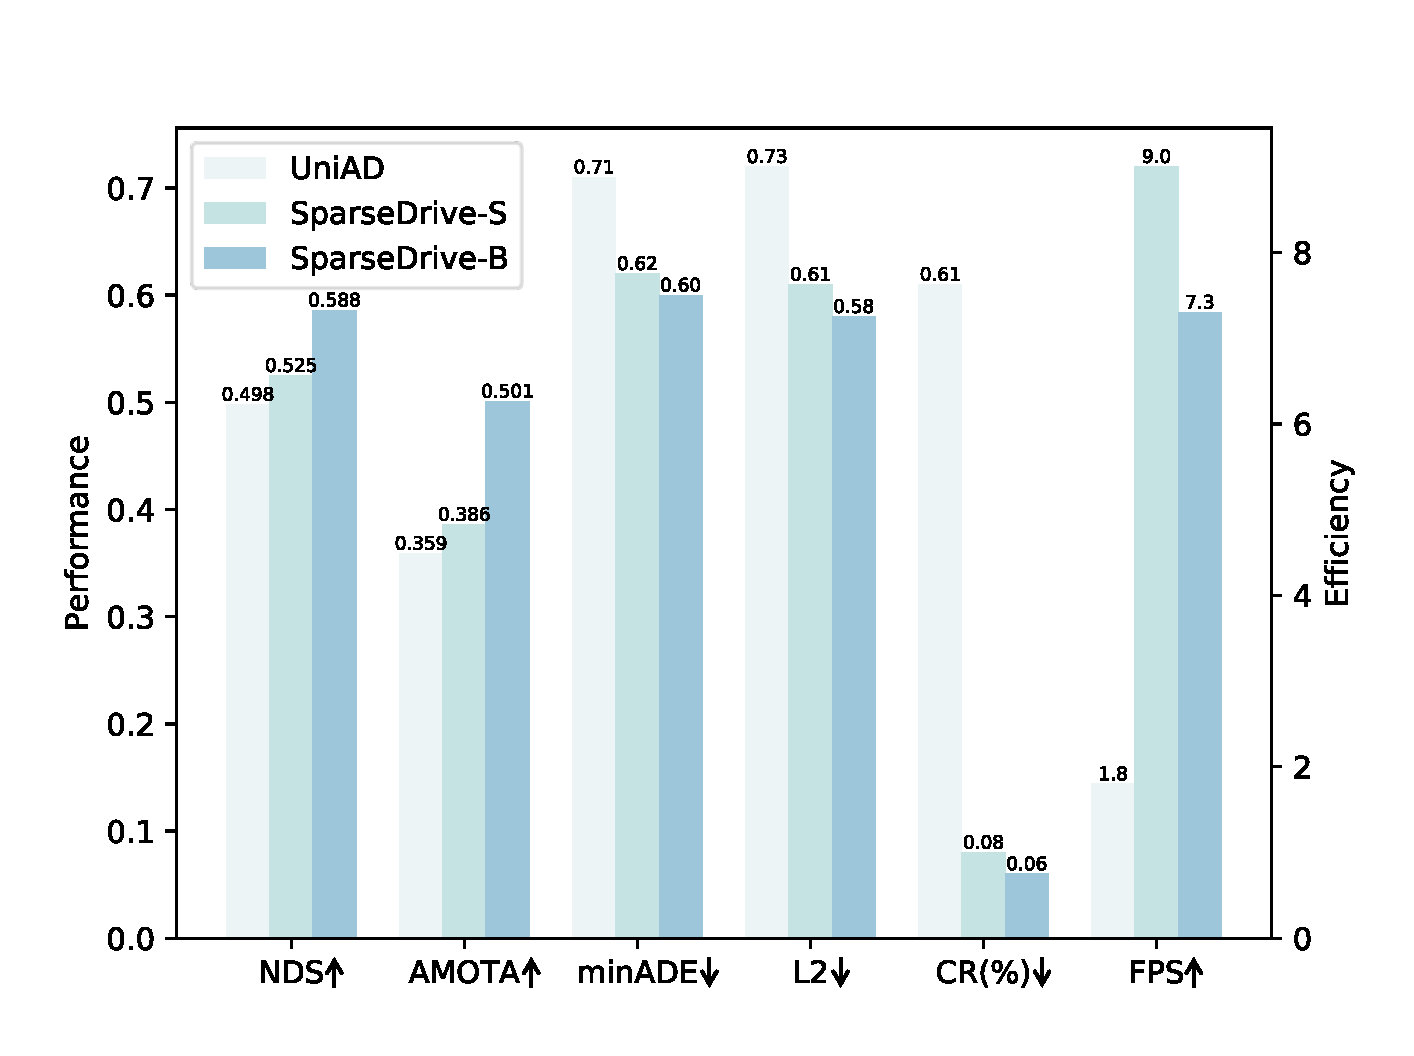
\includegraphics[width=1\linewidth]{Figures/comp.pdf}
    \caption{Comparison between our method and privous SOTA\cite{uniad}.}
    \label{fig:comp}
    \end{subfigure}
    \\
    \begin{subfigure}{1\linewidth}
    \end{subfigure}
    \\
    \begin{subfigure}{1\linewidth}
    \end{subfigure}

  \end{subfigure}
  
  \caption{The comparison of various end-to-end paradigms. (a) The BEV-Centric paradigm. (b) The proposed Sparse-Centric paradigm. (c) Performance and efficiency comparison between (a) and (b).}
  \label{fig:pipeline}
\end{figure}

Traditional autonomous driving system is characterized as
modular tasks in sequential order. While advantageous in interpretation and error tracking, it inevitably leads to information loss and accumulative errors across successive modules, thereby limiting the optimal performance potential of the system.

Recently, an end-to-end driving paradigm emerged as a promising research direction. This paradigm integrates all tasks into one holistic model, and can be optimized toward the ultimate pursuit for planning. However, the existing methods\cite{uniad, vad} are not satisfactory in terms of performance and efficiency. On one hand, previous methods rely on computationally expensive BEV features. On the other hand, the straightforward design for prediction and planning limits the model performance. We summarize previous 
methods as BEV-Centric paradigm in Fig. \ref{fig:pipeline_bev}.

To fully leverage the potential of end-to-end paradigm, we review the task design of existing methods, and argue that three main parallels shared between motion prediction and planning are neglected as follows: (1) Aiming at predicting future trajectories of surrounding agents and ego vehicle, both motion prediction and planning should consider the high-order and bidirectional interactions among road agents. However, previous methods typically adopt a sequential design for motion prediction and planning, ignoring the impact of ego vehicle on surrounding agents. (2) Accurate prediction for future trajectories requires semantic information for scene understanding, and geometric information to predict future movement of agents, which is applicable to both motion prediction and planning. While these information are extracted in upstream perception tasks for surrounding agents, it is overlooked for ego vehicle. (3) Both motion prediction and planning are multi-modal problems with inherent uncertainty, but previous methods only predict deterministic trajectory for planning. 

To this end, we propose SparseDrive, a Sparse-Centric paradigm as shown in Fig. \ref{fig:pipeline_sparse}. Specifically, SparseDrive is composed of a symmetric sparse perception module and a parallel motion planner. With the decoupled instance feature and geometric anchor as complete representation of one instance (a dynamic road agent or a static map element), \textbf{Symmetric Sparse Perception} unifies detection, tracking and online mapping tasks with a symmetric model architecture, learning a fully sparse scene representation. In \textbf{Parallel Motion Planner}, a semantic-and-geometric-aware ego instance is first obtained from ego instance initialization module. With the ego instance and surrounding agent instances from sparse perception, motion prediction and planning are conducted simultaneously to get multi-modal trajectories for all road agents. To ensure the rationality and safety for planning, a hierarchical planning selection strategy that incorporating a collision-aware rescore module is applied to select the final planning trajectory from multi-modal trajectory proposals.

With above effective designs, SparseDrive unleashes the great potential of end-to-end autonomous driving, as shown in Fig. \ref{fig:comp}. Without bells and whistles, our base model, SparseDrive-B, greatly reduces the average L2 error by 19.4\% (0.58m vs. 0.72m) and collision rate by 71.4\% (0.06\% vs. 0.21\%). Compared with previous SOTA (state-of-the-art) method UniAD\cite{uniad}, our small model, SparseDrive-S achieves superior performance among all tasks, while running 7.2$\times$ faster for training (20 h vs. 144 h) and 5.0$\times$ faster for inference (9.0 FPS vs. 1.8 FPS).
  
The main contribution of our work are summarized as follows:
\begin{itemize}[leftmargin=*]
\item We explore the sparse scene representation for end-to-end autonomous driving and propose a Sparse-Centric paradigm named SparseDrive, which unifies multiple tasks with sparse instance representation.
\item We revise the great similarity shared between motion prediction and planning, correspondingly leading to a parallel design for motion planner. We further propose a hierarchical planning selection strategy incorporating a collision-aware rescore module to boost the planning performance.
\item On the challenging nuScenes\cite{nuscenes} benchmark, SparseDrive surpasses previous SOTA methods in terms of all metrics, especially the safety-critical metric collision rate, while keeping much higher training and inference efficiency.
\end{itemize}